\chapter{Introduction}
3D Reconstruction and understanding are two fundamental problems for many applications in computer graphics, vision and robotics community. The wide availability of consumer range cameras has spurred extensive research in geometric reconstruction of real-world objects and scenes, with state-of-the-art 3D reconstruction approaches now providing robust camera tracking and 3D surface reconstruction~\cite{newcombe2011kinectfusion,izadi2011kinectfusion,whelan2015elasticfusion,dai2017bundlefusion}. However, producing photorealistic models of real-world environments requires not only geometric reconstruction but also high-quality color texturing.
Unfortunately, due to noisy input data, poorly estimated surface geometry, misaligned camera poses, unmodeled optical distortions, and view-dependent lighting effects,  aggregating multiple real-world images into high-quality, realistic surface textures is still a challenging problem. We aim at addressing this problem by minimizing color inconsistency or jointly optimizing the texture with a learned metric, as described in section~\ref{intro:texture-recon}.

On the other hand, understanding the 3D semantics of the scanned scenes is also a relatively open research problem. There has been a lot of recent works on semantic segmentation of 3D data using convolutional neural networks (CNNs). The advantage of these approaches over 2D image-based methods is that convolutions operate directly on 3D data, and thus are relatively unaffected by view-dependent image effects, such as perspective, occlusion, lighting, and background clutter.   However, the resolution of current 3D representations is generally quite low (2cm is typical), and so the ability of 3D CNNs to discriminate fine-scale semantic patterns is usually far below their color image counterparts \cite{long2015fully,he2017mask}. We propose to address this issue by firstly solve the canonical surface parameterization problem (section~\ref{intro:param}), and design a novel convolutional neural network that directly operates on the 3D surface based on the parameterization (section~\ref{intro:texture-learn}). Finally, we observe the existence of high correlation between the canonical frames from the surface parameterization and the RGB signals on the texture, and thus propose to estimate the local canonical surface frames from RGB images (section~\ref{intro:frame}).


\section{Texture Reconstruction}
\begin{figure}
    \centering
    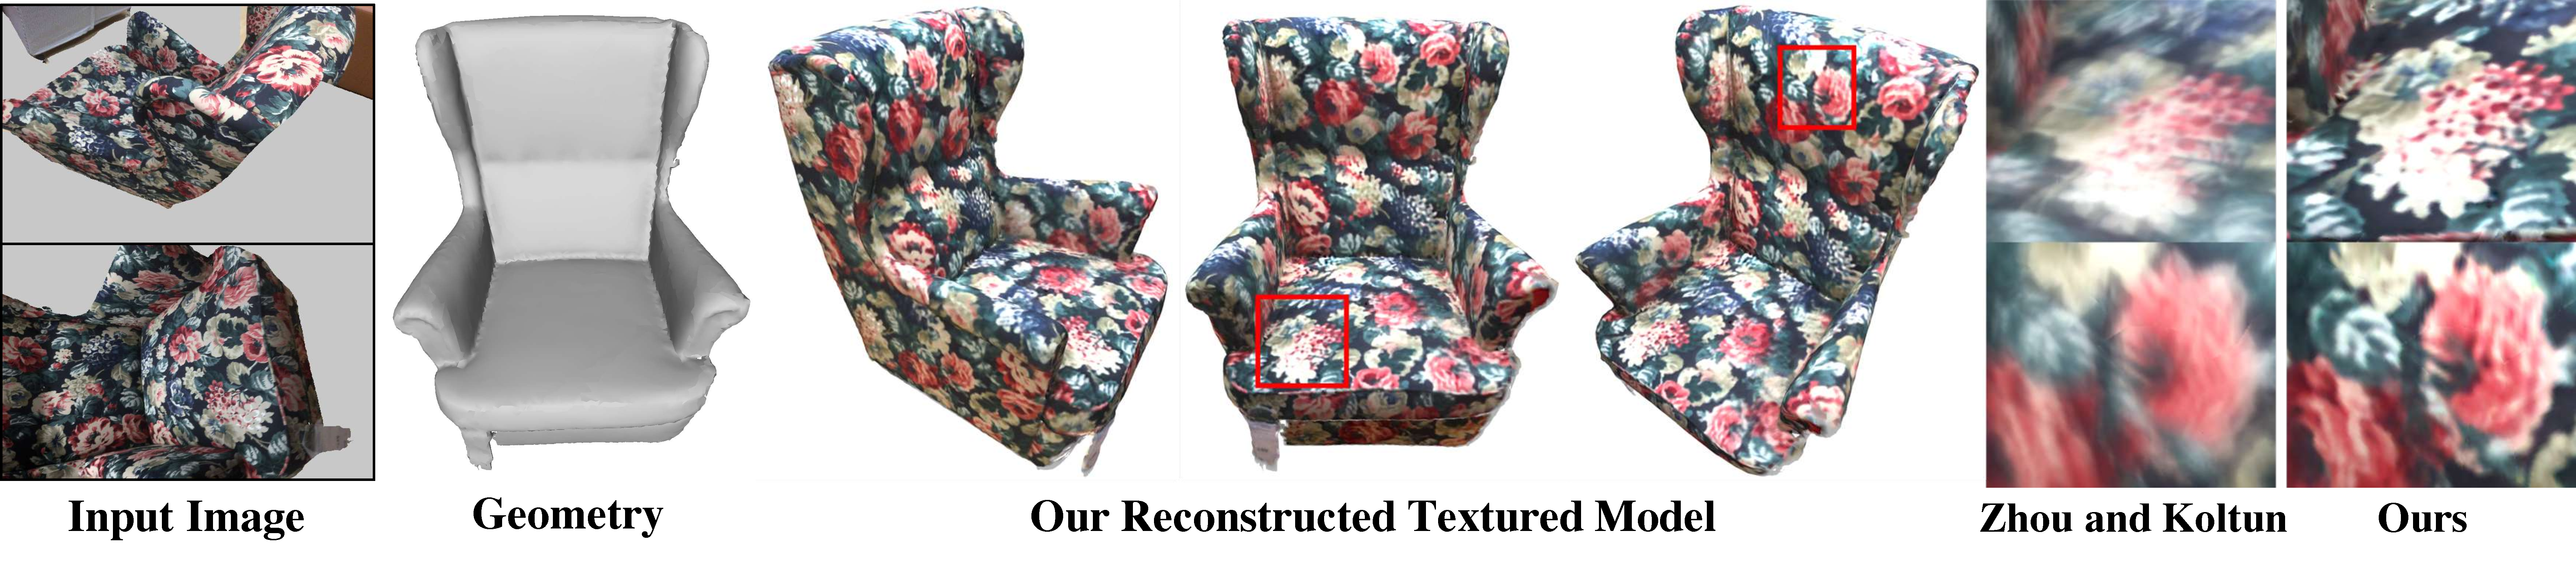
\includegraphics[width=\textwidth]{texturegen/figures/teaser-n.pdf}
    \caption{Our goal is to reconstruct high-quality textures from the 3D scan with aligned input images. Traditional optimize for a parametric color map to reduce misalignment error (Zhou and Koltun~\cite{zhou2014color}). We seek better color consistency optimization and view aggregation method, and further derive a flexible texture optimization framework based on a learned metric that is robust to common scanning errors.}
    \label{fig:toptim-teaser}
\end{figure}

\label{intro:texture-recon}
\paragraph*{Motivation}
RGB-D scanning has made rapid advances in recent years with the introduction of commodity range sensors, such as the Microsoft Kinect, Intel RealSense, or Google Tango.
State-of-the-art online and offline 3D reconstruction methods now allow remarkable capture and digitization of a variety of real-world environments, with faithful geometric fidelity~ \cite{newcombe2011kinectfusion,izadi2011kinectfusion,chen2013scalable,niessner2013real,choi2015robust,dai2016bundlefusion}.
Although the intended applications of these methods cover a variety of gaming, virtual reality, and augmented reality scenarios, the quality of the resulting 3D models remains far from the caliber of artist-modeled content.
In particular, current reconstructions still suffer from noise, oversmoothing, and holes, rendering them inadequate for use in production applications.

In many graphics applications, we observe that the surface textures are more important to visual perception than geometry; for instance, many video games make use of techniques such as billboarding or bump mapping~\cite{decoret1999multi}
to achieve high-detail visuals at low cost, with almost imperceptible difference to using accurate geometry.
Unfortunately, the color quality of existing 3D reconstruction methods often suffers from artifacts due to motion blur and rolling shutter from commodity color cameras. 
This is compounded by oversmoothing and camera pose micro-misalignments due to popular reconstruction techniques.
For instance, the seminal volumetric fusion work~\cite{curless1996volumetric} is commonly used to generate a 3D model from input RGB-D frames by performing a weighted average over projected depth and color observations.
While effectively regularizing out noise, this also results in oversmoothed geometry and color.
Additionally, since camera poses are computed from imperfect color and noisy, relatively low-quality depth, they often suffer from micro-drift, which further exacerbates resulting visual artifacts such as ghosting and oversmoothing. In order to overcome these problems, various approaches have been developed to optimize color textures using models to adjust camera poses~\cite{zhou2014color}, distort images~\cite{bi2017patch,zhou2014color}, and balance colors \cite{zhou2014color}.  However, these prior approaches are not expressive enough and/or their optimization algorithms are not robust enough to handle the complex distortions and misalignments commonly found in scans with commodity cameras -- and therefore they fail to produce high-quality results for typical scans as shown in the results from Zhou and Koltun~\cite{zhou2014color} in Figure~\ref{fig:toptim-teaser}.
 To address these issues, we propose to seek better color consistency optimization and view aggregation method, and further derive a flexible texture optimization framework based on a learned metric that is robust to common scanning errors (right side of Figure~\ref{fig:texturenet-teaser}).

For effective use in gaming, VR, or AR applications, reconstructed environments must not have holes, which are always present in real-world scans, due to occlusions.
Thus, we propose to facilitate the high-quality texture mapping on a relatively simple geometric representation of a object or scene using CAD model or primitive abstraction.

\paragraph*{Texture Reconstruction and Primitive Abstraction}
We propose \emph{3DLite}~\cite{huang20173dlite} as an approach to generate lightweight, complete, CAD-like models with high-quality textures of large-scale indoor scenes.
We take as input an RGB-D video sequence from a handheld commodity sensor, and first reconstruct the scene with existing 3D reconstruction methods.
Since we aim to generate complete scenes and sharp, clean textures, we employ a primitive-based abstraction to represent the scanned environments.
In particular, we use plane primitives, as planes facilitate texture mapping as well as scene completion through extrapolation, thus generating a denoised geometric representation of the scene.
We first optimize for these primitives under a Manhattan assumption, since man-made environments are often designed in such highly structured fashion.
In order to complete the scene geometry in occluded regions, we formulate a new hole-filling approach by extrapolating the planar primitives according to unknown space as seen by the camera trajectory.
That is, we respect the known empty space in the scene and only fill holes in regions unseen by the camera.
This generates a complete geometric representation of the scene.
We then perform a novel texture optimization to map the scene geometry with sharp colors from the input RGB data.
To generate complete textures for the entire scene, we follow this with a texture completion in unseen, hole-filled regions.
Since camera poses estimated from noisy RGB-D data are prone to micro-drift, our texture optimization step solves for refined rigid and non-rigid image alignments, optimizing for photo-consistency using both sparse color and dense geometric information.
To mitigate the effects of motion blur and auto-exposure, we perform an exposure correction, and select and stitch together only the sharpest regions of the input RGB images, obtaining globally consistent, sharp colors.
Finally, for regions which lack color due to occlusions in the input scan, we inpaint the texture using color information from similar textures in the scene.

\begin{figure}
    \centering
	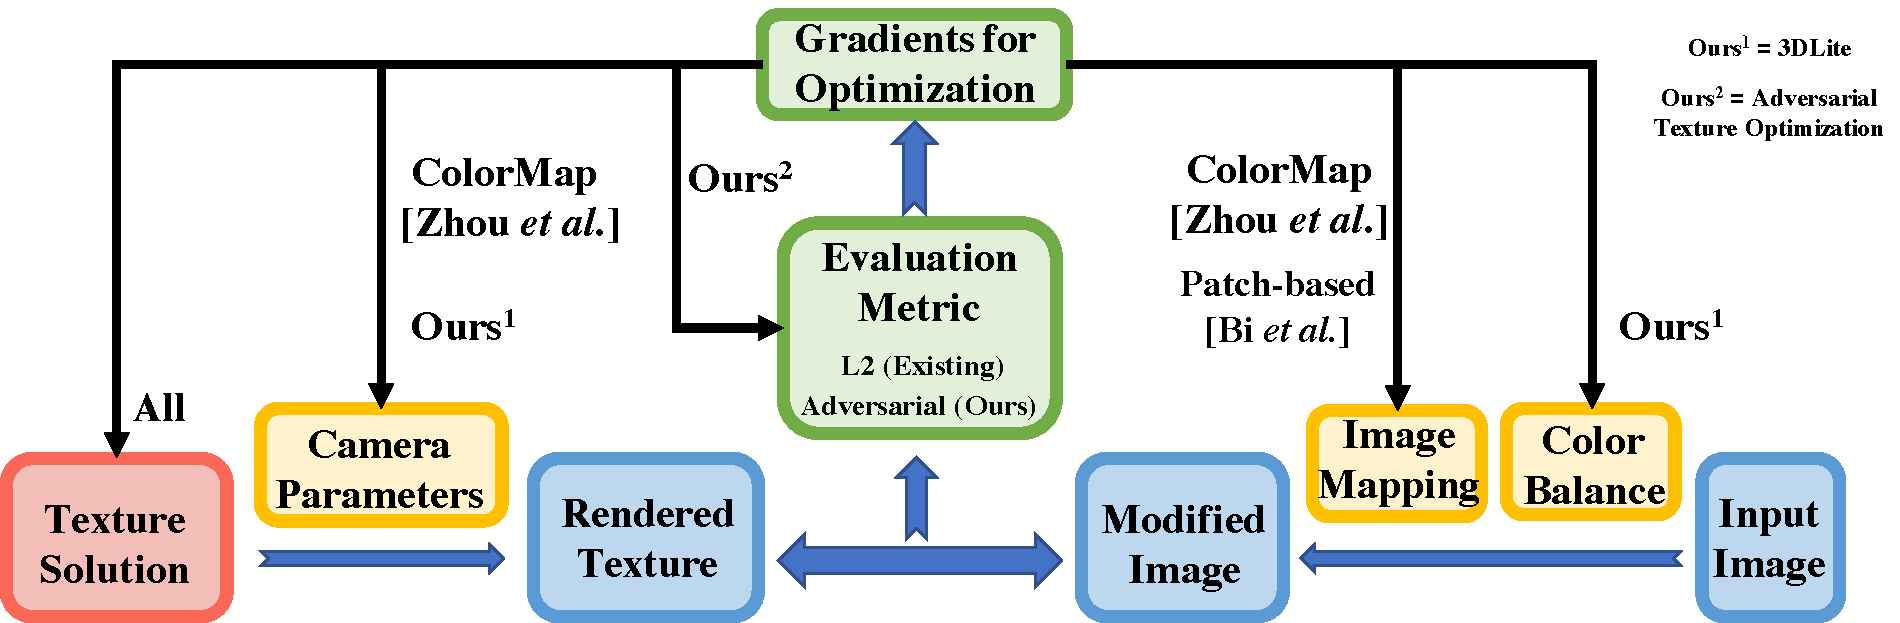
\includegraphics[width=\linewidth]{texturegen/figures/concept.pdf}
	\caption{All methods target at optimizing a texture solution. Existing methods optimize the texture jointly with camera parameters~\cite{zhou2014color,huang20173dlite}, image mapping~\cite{zhou2014color,bi2017patch} or color balance~\cite{huang20173dlite}. Instead, we jointly solve texture with an adversarial evaluation metric to tolerate the errors.}
	\label{fig:toptim-concept}
\end{figure}

\paragraph*{Adversarial Metric for Texture Optimization}
Prior approaches depend on explicit models and color consistency optimization, and are not expressive enough and/or their optimization algorithms are not robust enough to handle the complex distortions and misalignments commonly found in scans with commodity cameras.

To address these issues, we propose a flexible texture optimization framework based on a learned metric that is robust to common scanning errors.
% the scanning errors tuned separately for each individual scan. 
 The key idea behind our approach is to account for misalignments in a {\em learned objective function} of the texture optimization.   
 Rather that using a traditional object function, like $L1$ or $L2$, we learn a new objective function (adversarial loss) that is robust to the types of misalignment present in the input data.  This novel approach eliminates the need for hand-crafted parametric models for fixing the camera parameters \cite{zhou2014color,huang20173dlite} or image mapping \cite{bi2017patch,zhou2014color} or color balance \cite{huang20173dlite} (bottom row of Figure~\ref{fig:toptim-concept}) and replaces them all with a learned evaluation metric (green box in Figure~\ref{fig:toptim-concept}).   As such, it adapts to the input data.
 
Inspired by the success of adversarial networks in image synthesis~\cite{goodfellow2014generative}, we propose to use a learned conditional discriminator to serve our {\em objective function}, and jointly optimize the color texture of a reconstructed surface with this discriminator.
The condition is a captured image $I_A$ from the source view $V_A$, and the query is either (i) ``real:'' a second captured image $I_B$ (from an auxiliary view $V_B$) projected onto the surface and then rendered back to $V_A$, or (ii) ``fake:'' an image of the optimized synthetic texture rendered to view $V_A$. By optimizing the surface texture while jointly training this conditional discriminator, we aim to produce a texture that is indistinguishable from reprojections of captured images from all other views.  
%
During the optimization, the discriminator learns invariance to the misalignments and distortions present in the input dataset, while recognizing synthetic artifacts that do not appear in the real images, like local blurs and seams.  The synthesized textures optimized to fool the discriminator appear more realistic than in previous approaches.

Our experiments show that our adversarial optimization framework produces notably improved performance compared to state-of-the-art methods, both quantitatively on synthetic data and qualitatively on real data. 
Moreover, since it tolerates gross misalignments, we are able to generate realistic textures on CAD models which have been only roughly aligned to 3D scans, in spite of large mismatches in surface geometry. 
This opens up the potential to produce CAD models with realistic textures for content creation.

\section{Quadrangulation for Surface Parameterization}
\label{intro:param}
Surface parameterization serves as a fundamental step towards 3D surface learning with 2D convolutional neural networks. While 2D convolution has been widely used in image tasks, it is not well-applied in 3D surfaces. The key difference between 2D images and 3D surfaces is that image coordinate system serves as a consistent global definition of how the 2D domain is parameterized, while there is no global consistent definition of surface parameterization in 3D. Thus, we target at first solving the problem of the seamless surface parameterization, which is closely related to the quadrangulation problem in the geometry processing community.

State-of-the-art algorithms for quadrilateral surface meshing typically compute, as a first step, an \emph{orientation field} that assigns local coordinate axes to some points on the input surface \cite{knupp1995mesh,ray2006periodic,kalberer2007quadcover,bommes2009mixed}. The {\em Instant Field-Aligned Meshes} \mbox{algorithm} of Jakob et al.~\cite{jakob2015instant} subsequently computes a \emph{position field} that assigns local coordinates %(in the frame of the local coordinate axes)%
to those points. The orientation field determines the directions of the edges of a quadrilateral mesh, and the position field determines where the mesh vertices are placed. Ideally, both fields should vary smoothly over the surface, while obeying constraints that help to align the mesh with the sharp edges and the curvature of the object.
%(These fields provide some of the utility one would expect from having a parametrization of the surface, but they can adapt more easily to strangely shaped objects than a traditional mapping from a rectangle can.)

Both types of field can have irregularities called \emph{singularities}. If the fields are defined continuously over the surface, a singularity is a region where one of the fields is not locally smooth.
%(We will work with the discrete analogs of singularities for ``fields'' defined on the vertices of a triangular mesh.)
%Typically, there are reasons why the field cannot be locally smooth everywhere; the effort to compute smooth fields tends to produce singularities only where it is difficult not to produce them.
The pitfall of these singularities is that the quad mesh subsequently produced is likely to have an \emph{irregular vertex}---a vertex whose valence is not 4---near the singularity. 
%For a smooth surface with no sharp edges, every vertex in an ideal quadrilateral mesh would have valence 4, but this ideal is rarely attainable. (Every quadrilateral mesh with the topology of a sphere must have at least eight vertices of valence 3 if no vertex is permitted a valence less than 3---think of a cube---but in a mesh of a torus every vertex can have degree 4.)
Unfortunately, irregular vertices can cause problems for applications; for instance, they cause unsightly visual artifacts in Catmull--Clark subdivision, or additional work for an artist to edit a model.
%(because the subdivision surface is only $C_1$-continuous at these vertices rather than $C_2$-continuous).

% \olga{I think this whole previous paragraph is rather muddled. If the point it's trying to make is that too many singularities are undesired, I'd try saying something along the following lines: a) the methods that do quad meshing via a field are based on global parameterization. Namely, once the field is computed, the field directions are prescribed as gradients of two (u,v) functions defined everywhere on the mesh, such that the entire mesh can be mapped to the plane using those two functions. Then, the integer grid lines on the u,v plane are mapped back onto the mesh and this yields a grid-like pattern, or quadrangulation. b) Since the global parameterization involves mapping a non-disk-topology (non-flat) surface onto the (flat, zero curvature) plane, singularities are necessary to accumulate the curvature so that the mapping is zero-curvature everywhere *but* at the singularities. Additional singularities can appear in the field depending on how non-flat the input surface is. However, the distortion of the mapping is typically accumulated around singularities, and (as you say) singularities mean irresular vertices in the quad mesh, which relates to subdivision surface smoothness, so typically it is desirable to control their number.}

Algorithms that rely purely on local mesh computations are fast, but they produce meshes with many singularities. It is possible to modify the fields to move singularities and sometimes even to eliminate them; but eliminating a singularity
%(if it isn't merely gratuitous nonsmoothness)
usually involves merging pairs of singularities located all around the geometry, which is ``nonlocal.'' 
%Analogously, if a quad mesh has a vertex of valence 3 and a vertex of valence 5, it is sometimes possible to modify the mesh so both vertices have valence 4 without changing the valences of the other vertices, but this modification must change (at the very least) a whole strip of quadrilaterals joining the two irregular vertices. 
%The most effective quad meshers take a global view of the surface when they try to minimize the number of singularities, but this can make them quite slow. By contrast, algorithms that rely purely on local mesh computations are fast, but they produce meshes with many more singularities.
% \olga{ Global methods are global -- they don't exactly rely on local propagation of singularities of the strip-type that is mentioned above (although this is sometimes done as postprocessing), so this reads a bit odd. I'd say that global methods optimize for singularities in one go depending on mesh curvature and the desired field alignment to features, so in a way they distribute the curvature better, but are slow -- local methods exist that are faster , but since they don't take into account the entire surface at once, they can greedily introduce many singularities to zero-out the curvature. In both cases, some level of singularity editing/merging might be possible, via some mostly greedy local-propagation steps}.
A global view of quad meshing taken by Bommes et al.~\cite{bommes2009mixed}, who cast the problem of seamless global parametrization as a mixed-integer constrained optimization problem (MIP).
%They also use a MIP to cut the surface and define a global parametrization of the cut surface (related to the position field we discuss, but with important differences). 
The method produces quadrilateral surface meshes of very high quality, but it is slow and it does not scale well to large meshes. By contrast, the much more efficient Instant Meshes algorithm of Jakob et al.~\cite{jakob2015instant} uses local smoothing operators to compute an orientation field and a position field quickly. Their method is scalable and produces high quality quad-dominant meshes without much distortion. However, it may produce singularities in the position field in addition to singularities in orientation field.

We present \emph{QuadriFlow}~\cite{huang2018quadriflow}, a scalable, robust algorithm for automatic quad meshing that builds upon Instant Meshes but uses a global method to remove all the singularities from the position field.
%, while it is theoretically impossible to remove all the singularities from the orientation field due to surface topological constraints.}
We do not change the orientation field, which typically has many fewer singularities. Our method solves a minimum cost network flow problem as a subproblem, for which efficient algorithms are available. The speed and reliability of our algorithm can enable designers to work on a modeling task interactively and extract a quad mesh in less than a second for tens of thousands of faces, and enable physical simulations to perform per-timestep remeshing updates. Our current implementation is a \emph{remeshing} algorithm, meaning that its input is a triangular mesh of the input surface (like many other quad meshing algorithms), though it could be modified to take a point cloud input as Instant Meshing does.

We view singularity-free position field computation as a globally constrained optimization problem.
%whose solution involves three main components. We begin as Jakob et al.\ do,
%(in fact, we use their code)
%computing the position field by minimizing a mixed-integer energy function. Second, we introduce additional regularity constraints on the integer variables to remove singularities from the position field. Third, we remove inverted triangles by imposing orientation constraints. 
Unlike Bommes et al., we do not solve the problem by mixed-integer programming. Instead, we split it into three stages.
\begin{itemize}
\item Compute the orientation and position fields just as Jakob et al.\ do, without enforcing additional constraints.
\item Enforce our constraints by modifying only the integer variables of the position field, changing the integers as little as possible.
\item Re-optimize the continuous variables of the position field with the integer variables held fixed.
\end{itemize}
The third stage is not difficult, requiring the solution of a linear system. Our main contribution is a fast and effective method for the second, largely combinatorial stage. Because of the regularity constraints, the second stage is a mixed-integer programming problem, for which it is NP-hard to find an optimal solution, but we can obtain good approximate solutions in practice. We reduce the problem to an integer linear program (ILP). We approximate the ILP as an easier \emph{minimum cost network flow} (MCF) problem, which can be solved in polynomial time~\cite{klein1967primal}. We further improve the efficiency by a multi-resolution algorithm. To enforce consistent triangle orientations (no inverted triangles), we impose a set of quadratic inequality constraints. We are able to satisfy most of these constraints through simple greedy edge contractions; we find we can satisfy most of the remaining difficult ones by locally solving a small boolean satisfiability problem (SAT).

By replacing the MIP solver with an MCF solver that globally reduces the number of singularities, plus edge contractions and a SAT solver that locally impose triangle orientation constraints, we obtain a scalable quad remesher that produces many fewer singularities than Instant Meshes, often by a factor of four, while being much faster than the method of Bommes et al. QuadriFlow remeshes a one-million triangle mesh in 5 seconds, which is comparable to the interactive method of Ebke et al.~\cite{ebke2016interactively}. Our meshes have less distortion compared to other global methods, and rarely suffer from nonmanifold structure or holes, thanks to the consistent orientation constraints. In a test on 17,000$+$ surfaces created from ShapeNet~\cite{chang2015shapenet}, %,huang2018robust
QuadriFlow robustly removed all the singularities from every discrete position field.


\section{Texture Understanding}
\subsection{Semantics from Texture}
\begin{figure}
	\begin{center}
		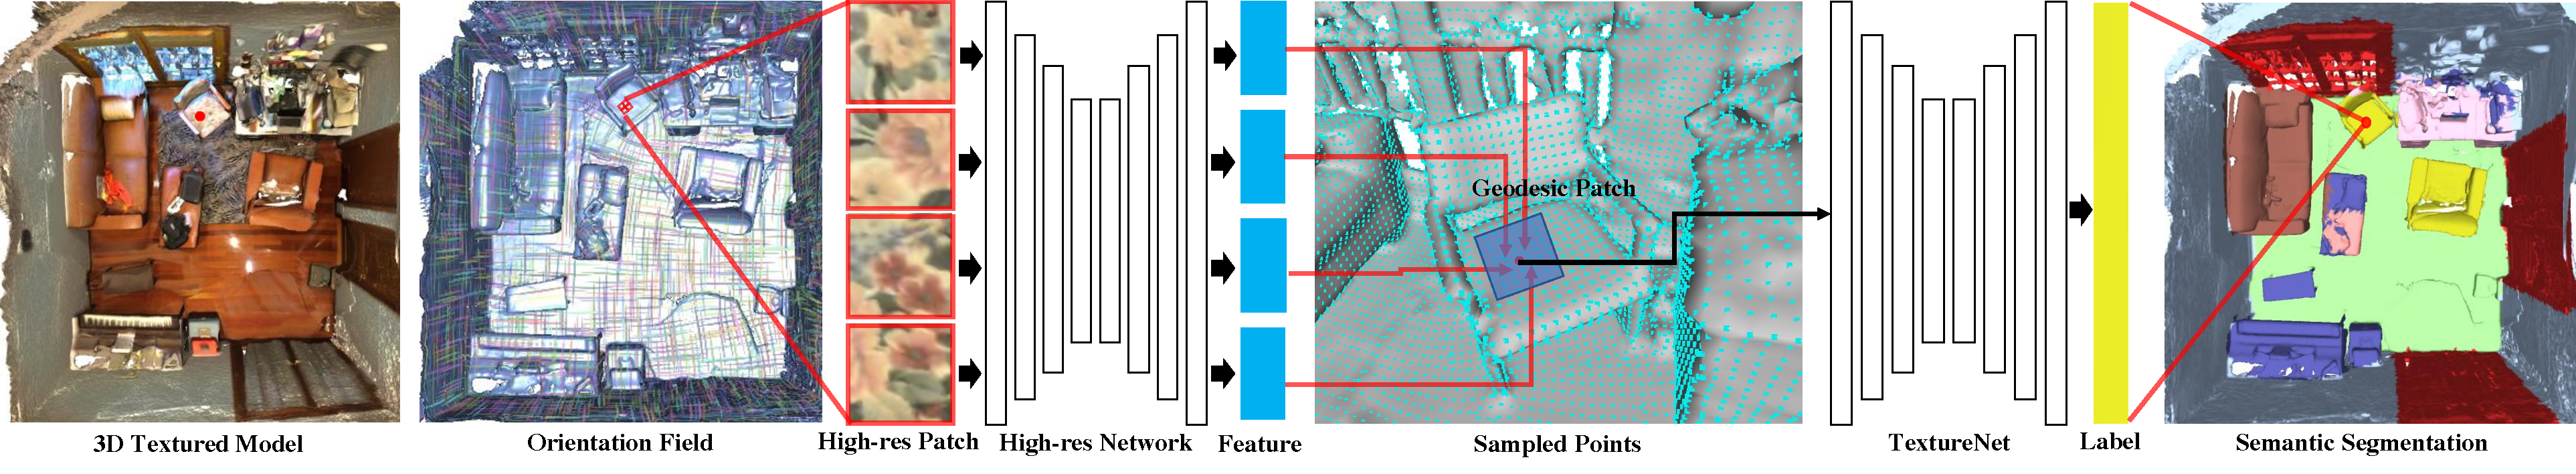
\includegraphics[width=\linewidth]{texturenet/teaser/teaser.pdf}
		\caption{TextureNet takes as input a 3D textured mesh.  The mesh is parameterized with a consistent 4-way rotationally symmetric (4-RoSy) field, which is used to extract oriented patches from the texture at a set of sample points.   Networks of 4-RoSy convolutional operators extract features from the patches and used for 3D semantic segmentation.}
		\label{fig:texturenet-teaser}
	\end{center}    
\end{figure}
\label{intro:texture-learn}
Though existing methods are now able to reconstruct textured 3D meshes suitable for visualization, understanding the 3D semantics of the scanned scenes from these high-resolution signals is still a relatively open research problem. 

To address the efficiency of 3D convolution, we propose a new convolutional neural network, \emph{TextureNet}~\cite{huang2018texturenet}, with a 2D convolution kernel that extracts features directly from high-resolution signals associated with 3D surface meshes.  Given a map that associates high-resolution signals with a 3D mesh surface (e.g., RGB photographic texture), we define convolutional filters that operate on those signals within domains defined by geodesic surface neighborhoods.   This approach combines the advantages of feature extraction from high-resolution signals (as in \cite{dai20183dmv}) with the advantages of view-independent convolution on 3D surface domains (as in \cite{tatarchenko2018tangent}).
This combination is important for the example in labeling the chairin Figure \ref{fig:texturenet-teaser}, whose surface fabric is easily recognizable in a color texture map.

During our investigation of this approach, we had to address several research issues, the most significant of which is how to define on geodesic neighborhoods of a mesh.   One approach could be to compute a global UV parameterization for the entire surface and then define convolutional operators directly in UV space; however, that approach may induce significant deformations due to flattening, not always follow surface features, and/or produce seams at surface cuts.  Another approach could be to compute UV parameterizations for local neighborhoods independently; however, then adjacent neighborhoods might not be oriented consistently, reducing the ability of a network to properly learn orientation-dependent features.   Instead, we compute a 4-RoSy (four-fold rotationally symmetric) field on the surface using QuadriFlow~\cite{huang2018quadriflow} and define a new 4-RoSy convolutional operator that explicitly accounts for the 4-fold rotational ambiguity of the cross field parameterization. A 4-RoSy (four-way rotationally symmetric) field is a configuration of 4 orthogonal tangent directions associated with each vertex in the shape of a cross that varies smoothly over the mesh surface.  Since the 4-RoSy field from QuadriFlow has no seams, aligns to shape features, induces relatively little distortion, has few singularities, and consistently orients adjacent neighborhoods (up to 4-way rotations), it provides an attractive trade-off between distortion and orientation invariance.

Results on 3D semantic segmentation benchmarks show an improvement of the 4-RoSy convolution on surfaces over alternative geometry-only approaches (by 6.4\%), plus significantly further improvement when applied to high-resolution color signals (by 6.9-8.2\% ).  With ablation studies, we verify the importance of the consistent orientation of a 4-RoSy field and demonstrate that our sampling and convolution operator works better than other alternatives.

\subsection{Surface Parameterization from Texture}
\label{intro:frame}
The geometric surface parametrization serves not only as a basis for 3D convolution operators to apply, but also as useful information that is highly-correlated and learnable from the color signals in a single image.

In recent years, learning to predict 3D properties from a single RGB image has made great progress.  For example, monocular depth estimation~\cite{shelhamer2015scene,li2017two,xu2017multi,wang2018adaptive,fu2018deep} and surface normal prediction~\cite{eigen2015predicting,wang2015designing,bansal2016marr,qi2018geonet} have improved dramatically.  There are many applications for these tasks in scene understanding and robot interaction.

The main challenge in this domain is choosing an appropriate representation of 3D geometry to predict.  Zhang~\textit{et al.}~\cite{zhang2018deep} predict dense surface normals and then use geometric constraints to solve for depth with a global optimization.  GeoNet~\cite{qi2018geonet} predicts both surface normals and depth and then passes them to a refinement network for further optimization.  These methods are clever in their use of geometric constraints to regularize dense predictions.   However, they infer only 2 of the 3 degrees of freedom in a 3D coordinate frame -- the rotation in the tangent plane around the surface normal is left unknown.  As such, they are missing 3D information critical to many applications.   For example, they cannot assist an AR system in placing a picture frame on a wall or a laptop on a table because they don't know the full 3D coordinate frame (including tangent directions) of the wall or table surfaces.

 \begin{figure}
    \centering
    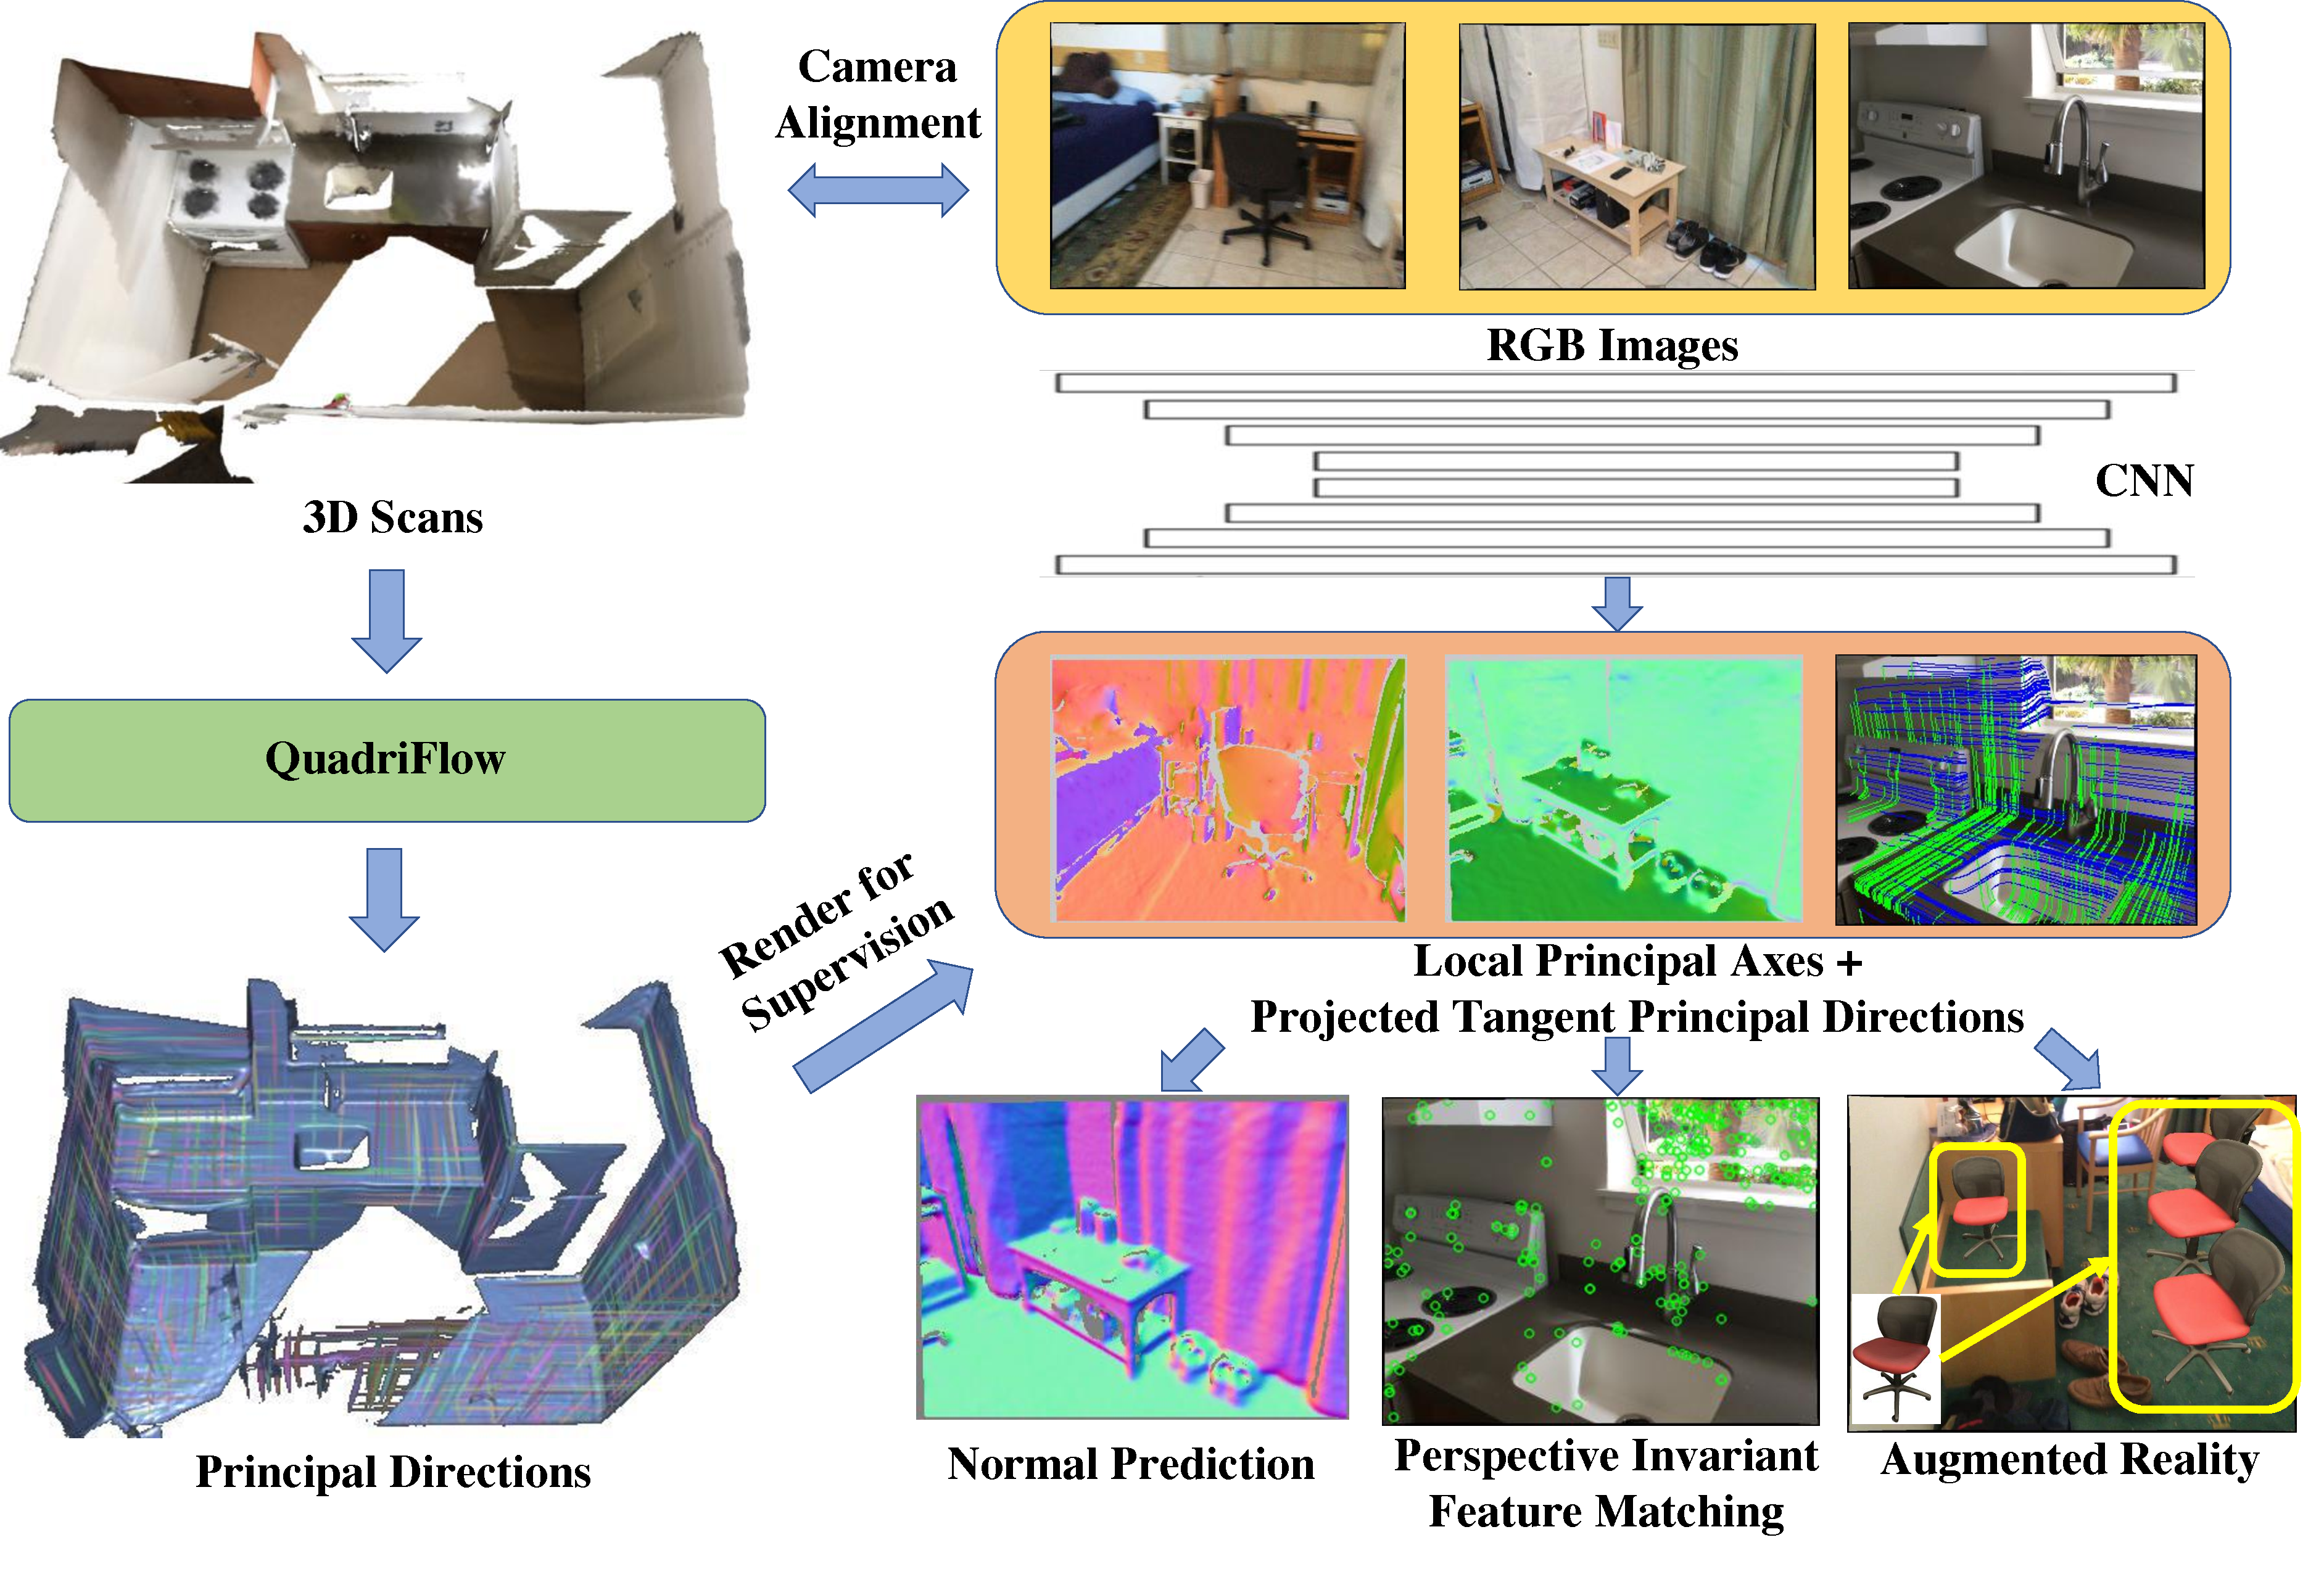
\includegraphics[width=0.75\linewidth]{FrameNet/graph/teaser.pdf}
    \caption{We propose the novel task of predicting dense 3D \cframe{} from a single RGB image. We compute the frames from reconstructed meshes using QuadriFlow and render them to images to supervise the task.  We train a network that predicts all directions of the frames jointly.  We find that predicted tangents provides better surface normals, and are useful for applications like feature matching and augmented reality.}
    \label{fig:framenet-teaser}
    \vspace{-0.1in}
\end{figure}


\cam{In this work, we propose FrameNet~\cite{framenet} as a novel image-to-3D task: dense 3D \cframe{} estimation from a single image (figure~\ref{fig:framenet-teaser})
.  This task requires predicting a full 3D coordinate frame defined by the surface normal {\em and two principal tangent directions} of the surface observed at every pixel in a RGB image.  We investigate this task for three reasons.   First, we expect that predicting principal tangent directions is easier than predicting normals because they are often aligned with observable patterns in surface textures (e.g., wood grains, fabric weaves, tile seams, etc.) and surface boundaries, which are directly observable in images %(figure~\ref{fig:framenet-vis-direction})
.  Second, we expect that joint surface normal and tangent prediction is more robust than normal prediction alone due to the regularization provided by orthogonality constraints.  Third, we expect that predicting a full canonical 3D coordinate frame at every pixel is useful for many applications, such as augmented reality.}

\cam{We have implemented an algorithm for this task in a supervised setting.   To acquire ``ground truth'' \cframe{}, we leverage data from RGB-D scanning datasets, like ScanNet~\cite{dai2017scannet}, which provide large sets of images posed within reconstructed 3D meshes.  
We compute \cframe{} on the meshes and render them to the RGB images to produce training data.  There are multiple choices for how to define the frames.  A simple approach would be to use Manhattan frames; however they
reflect only the global scene orientation %(figure~\ref{fig:framenet-vis-direction}(a))
.   Instead, we compute locally consistent 4-RoSy \cframe{} that follow principal curvatures using the Quadriflow algorithm~\cite{huang2018quadriflow} %(figure~\ref{fig:framenet-vis-direction}(b))
.  We find that the surface tangent directions computed this way are consistent with image features and can be learned by a network from 2D data.}

\cam{The \cframes{} are fundamental 3D properties of a scene, as they imply the canonical transformation that maps the 3D surface to the image plane.  They provide not only the surface normal, but also canonical tangent directions and their projections onto the image plane.  We show that predicting all these directions jointly can improve surface normal estimation, local patch description using SIFT features~\cite{lowe2004distinctive}, and allow the insertion of novel objects with correct orientation in augmented reality applications.}

\section{Contributions and Thesis Outlines}
This thesis mainly focuses on texture reconstruction and understanding. We discuss the related works in chapter~\ref{chapter:related}. Texture optimization is based on color consistency optimization~\cite{huang20173dlite} or joint adversarial metric optimization, as described in chapter~\ref{chapter:texture-recon}. For understanding, we first solve the fundamental surface parameterization problem~\cite{huang2018quadriflow} as explained in chapter~\ref{chapter:param}, and design a network with 2D convolution operators~\cite{huang2018texturenet} under the canonical surface parameterization (chapter~\ref{sec:texturenet}. Observing the correlation between surface parameterization and texture signals, we propose to learn canonical frames from RGB images~\cite{framenet} in chapter~\ref{sec:framenet}. Finally, we will conclude in chapter~\ref{chapter:conclude}.

Overall, the contributions of this thesis include:
\begin{itemize}
    \item We propose \emph{3DLite} as an approach to produce high-quality surface textures on top of the lightweight planar geometry abstracted from the scan.
    \item We propose an approach to produce photorealistic textures for approximate surfaces, even from misaligned images, by learning an objective function that is robust to scanning errors.
    \item We propose \emph{Quadriflow} as a scalable and robust quadrangulation algorithm that is solvable in polynomial time.
    \item Based on consistent local parameterizations from \emph{Quadriflow}, we design \emph{TextureNet} as a novel neural network for extracting features from high-resolution signals living on surfaces embedded in 3D.
    \item We observe the high correlation between surface parameterization from \emph{Quadriflow} and RGB signals on surface texture, and identify an important new 3D vision problem with a solution: local canonical frame estimation from RGB images.
\end{itemize}
